\subsubsubsubsection{Agent}
\begin{figure}[h]
\centering
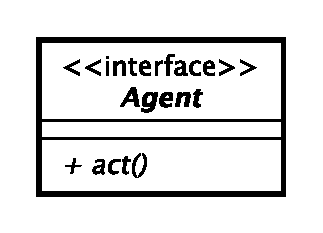
\includegraphics[scale=0.6,keepaspectratio]{images/solution/app/backend/agent.eps}
\caption{\pActive::Agent}
\label{fig:sd-app-agent}
\end{figure}
\FloatBarrier
\begin{itemize}
  \item \textbf{\descr} \\
    It represents an entity that moves through the city, consuming its 
route at each stretch treaded.
  \item \textbf{\ops}
  \begin{itemize}
    \item[+]  \texttt{\textit{act()}} \\
Activates the entity which sets its state to \textit{running} and 
starts consuming its route.
  \end{itemize}
\end{itemize}
